\documentclass[article,screen]{acmart}
\AtBeginDocument{%
  \providecommand\BibTeX{{%
    \normalfont B\kern-0.5em{\scshape i\kern-0.25em b}\kern-0.8em\TeX}}}

\setcopyright{acmcopyright}
\copyrightyear{2024}
\acmYear{2024}
\acmDOI{XXXXXXX.XXXXXXX}

%\acmConference[Conf '24]{
  %International Symposium on Spatial and Temporal Data
%}{
  %August 23--25, 2023
%}{
  %Calgary, Canada
%}
%  Uncomment \acmBooktitle if th title of the proceedings is different
%  from ``Proceedings of ...''!
%\acmBooktitle{
%SSTD '23: International Symposium on Spatial and Temporal Data, August 23--25, 2023, Calgary, Canada
%}
%\acmPrice{15.00}
%\acmISBN{978-1-4503-XXXX-X/18/06}

\usepackage{subcaption}
%% For algorithms...
\usepackage{algorithm}
\usepackage{algpseudocode}
\algnewcommand\algorithmicforeach{\textbf{for each}}
\algdef{S}[FOR]{ForEach}[1]{\algorithmicforeach\ #1\ \algorithmicdo}
\algnewcommand\algorithmicswitch{\textbf{switch}}
\algnewcommand\algorithmiccase{\textbf{case}}
\algdef{SE}[SWITCH]{Switch}{EndSwitch}[1]{\algorithmicswitch\ #1\ \algorithmicdo}{\algorithmicend\ \algorithmicswitch}
\algdef{SE}[CASE]{Case}{EndCase}[1]{\algorithmiccase\ #1}{\algorithmicend\ \algorithmiccase}
\algtext*{EndSwitch}
\algtext*{EndCase}

\setlength{\textfloatsep}{2pt plus 1.0pt minus 2.0pt}

\usepackage{tikz}
\usetikzlibrary{shapes, arrows}

\begin{document}

\title{Scalable Processing of Moving Flock Patterns}
\author{Andres Calderon-Romero}
\email{acald013@ucr.edu}
\affiliation{
  \institution{University of California}
  \country{USA}
  \city{Riverside}
}

\author{Petko Balakov}
\email{petko@esri.com}
\affiliation{
  \institution{Esri}
  \country{USA}
  \city{Redlands}
}

\author{Marcos Vieira}
\email{marcos@gmail.com}
\affiliation{
  \institution{Google}
  \country{USA}
  \city{San Francisco}
}

\author{Vassilis J. Tsotras}
\email{tsotras@cs.ucr.edu}
\affiliation{
  \institution{University of California}
  \country{USA}
  \city{Riverside}
}

\renewcommand{\shortauthors}{Calderon, et al.}

\begin{abstract}
This work presents a scalable approach for identifying moving flock patterns in large trajectory databases, addressing the inefficiencies in current techniques for handling large spatio-temporal datasets. A moving flock pattern refers to a group of entities that move closely together within a defined spatial radius for a minimum time interval. We focus on improving the state-of-the-art sequential algorithms, which is capable of detecting such patterns but suffers from high computational costs, particularly with large datasets. By leveraging distributed frameworks and utilizing spatial partitioning, the proposed solution aims to significantly reduce the time required for detecting flock patterns. We highlight the challenges of spatial and temporal joins in massive datasets and offer optimizations like partition-based parallelism and strategies for managing flock patterns that span multiple partitions. The paper presents an experimental evaluation using synthetic trajectory datasets, demonstrating that the proposed methods substantially improve scalability and performance compared to existing sequential algorithms.

\end{abstract}

\begin{CCSXML}
<ccs2012>
   <concept>
       <concept_id>10010147.10010169.10010170</concept_id>
       <concept_desc>Computing methodologies~Parallel algorithms</concept_desc>
       <concept_significance>500</concept_significance>
       </concept>
   <concept>
       <concept_id>10002951.10002952.10002971</concept_id>
       <concept_desc>Information systems~Data structures</concept_desc>
       <concept_significance>500</concept_significance>
       </concept>
   <concept>
       <concept_id>10010147.10010919.10010172.10003817</concept_id>
       <concept_desc>Computing methodologies~MapReduce algorithms</concept_desc>
       <concept_significance>500</concept_significance>
       </concept>
 </ccs2012>
\end{CCSXML}

\ccsdesc[500]{Computing methodologies~Parallel algorithms}
\ccsdesc[500]{Information systems~Data structures}
\ccsdesc[500]{Computing methodologies~MapReduce algorithms}

\keywords{Mobile patterns}
\maketitle

\section{Introduction}
Technological advances in the past few decades have triggered an explosion in the collection of spatio-temporal data.  The increasing popularity of GPS devices and smartphones, along with the emergence of new disciplines such as the Internet of Things (IoT) and high-resolution Satellite/UAS imagery, has made it possible to collect vast amounts of data with spatial and temporal components.

In tandem, interest in extracting valuable information from such large databases has also grown.  Spatio-temporal queries about popular places or frequent events remain useful, but there has been growing interest in more complex patterns.  In particular, patterns that describe the group behavior of moving objects over significant periods.  Moving cluster \cite{kalnis_discovering_2005}, convoys \cite{jeung_discovery_2008}, flocks \cite{gudmundsson_computing_2006} and swarm patterns \cite{li_swarm_2010} reveal how entities move together over a minimum time interval.

Applications for this type of information are both diverse and intriguing, particularly when dealing with trajectory datasets \cite{jeung_trajectory_2011, huang_mining_2015}. Case studies span various domains, including transportation system management and urban planning \cite{di_lorenzo_allaboard_2016}, as well as ecology \cite{la_sorte_convergence_2016}. For example, \cite{turdukulov_visual_2014} explores the identification of complex motion patterns to discover similarities in tropical cyclone paths. Similarly, \cite{amor_persistence_2016} investigates eye movement trajectories to understand the strategies people use during visual searches. Additionally, \cite{holland_movements_1999} tracks the behavior of tiger sharks along the coasts of Hawaii to gain insight into their migration patterns.

One particular pattern of interest is the moving flock pattern, which captures how objects move within close proximity for a given time period. Closeness is defined by a disk of a specified radius within which the entities must remain. Since this disk can be positioned anywhere, detecting such patterns is a non-trivial problem. In fact, \cite{gudmundsson_computing_2006} highlights that finding flock patterns where the same entities stay together over time is an NP-hard problem. To address this, \cite{vieira_2009} proposed the BFE algorithm, the first approach capable of detecting flock patterns in polynomial time.

Despite the increasing availability of data, current state-of-the-art techniques for mining complex movement patterns still struggle with the performance demands of large-scale spatial data. This work introduces a scalable approach designed to detect moving flock patterns in very large trajectory databases. By leveraging emerging trends in distributed frameworks for spatial operations we aim to significantly improve the speed and efficiency of detecting these patterns.

\section{Related work}
The recent increased use of location-aware devices (such as GPS, smartphones, and RFID tags) has enabled the collection of vast amounts of data with spatial and temporal components.  Several studies have focused on discovering and analyzing these types of datasets \cite{leung_knowledge_2010, miller_geographic_2001}.  In this area, trajectory datasets have emerged as an interesting field where diverse kind of patterns can be identified \cite{zheng_computing_2011, vieira_spatio-temporal_2013}.  For instance, researchers have proposed techniques to discover spatial motion patterns such as moving clusters \cite{kalnis_discovering_2005}, convoys \cite{jeung_discovery_2008} and flocks \cite{benkert_reporting_2008, gudmundsson_computing_2006}.  Specifically, \cite{vieira_2009} introduced BFE (Basic Flock Evaluation), an innovative algorithm designed to efficiently identify moving flock patterns in polynomial time across large spatio-temporal datasets.

A flock pattern is defined as a group of entities that move together over a specified time period \cite{benkert_reporting_2008}. The applications of such patterns are broad and diverse. For instance, \cite{calderon_romero_mining_2011} identifies moving flock patterns in iceberg trajectories to analyze their movement behavior and their relationship with changes in ocean currents.

The BFE algorithm provides an initial approach for detecting flock patterns. It begins by identifying disks with a predefined diameter ($\varepsilon$) where moving entities are sufficiently close at specific time instants. This operation is computationally expensive due to the large number of points and time instances to be analyzed, with a complexity of $\mathcal{O}(2n^2)$ per time. Although the algorithm leverages a grid-based index and a stencil to accelerate this process, the overall complexity remains high.

Both \cite{calderon_romero_mining_2011} and \cite{turdukulov_visual_2014} adopt a frequent pattern mining approach to enhance performance when combining disks across time instants. Similarly, \cite{tanaka_improved_2016} utilize plane sweeping techniques, binary signatures, and inverted indexes to further accelerate this process. However, these methods retain the core strategy of BFE for detecting disks at each time instant.

In contrast, \cite{arimura_finding_2014} and \cite{geng_enumeration_2014} employ depth-first algorithms to analyze the time intervals of individual trajectories and report maximal duration flocks. However, these methods are less effective for dense datasets or those that involve large numbers of entities per time step, as they struggle to scale efficiently in such conditions.

Given the high computational demands of flock pattern detection, it is not surprising that parallelism has been employed to improve performance. For example, \cite{fort_parallel_2014} use extreme and intersection sets to report maximal, longest, and largest flocks on GPUs, albeit with limitations imposed by the GPU's memory model.

Despite the increasing adoption of cluster computing frameworks, particularly those with spatial data capabilities \cite{eldawy_spatialhadoop_2014, yu_demonstration_2016, pellechia_geomesa_2015, xie_simba_2016}, significant advancements in this area remain limited. To the best of our knowledge, this work is the first to explore the detection of moving flock patterns in a scalable approach.

\section{Scalable Kd-tree Partitioner with Dangle and Cut Edges Integration} \label{sec:extension_methods}

\subsubsection{Kd-tree Partition Strategy} %\label{sec:kdtreestrategy}
In Section \ref{sec:pstrategies}, we use the quadtree spatial index as the baseline for our partitioning strategy. The quadtree follows a space-oriented approach, as it does not consider the content of each cell when determining potential splits. In contrast, kd-tree-based partitioning employs a data-oriented approach by sorting and selecting the midpoint within a cell to guide the placement of splits for future child nodes.

Building and populating the kd-tree partitioning follows a process similar to that of the quadtree. First, a kd-tree is constructed from a sample representing 1\% of the input data to define the tree’s structure, where the leaves represent the partition’s cells. The input data is then fed into this kd-tree structure, with each edge assigned to the leaf cell containing its boundaries. After partitioning, the local DCELs for each layer are constructed, and the overlay operation is performed within each cell as described in Section \ref{sec:pstrategies}.

Section \ref{sec:extension_experiments} will compare two partitioning strategies, the one presented in \ref{sec:pstrategies} based on the quadtree (i.e. space-oriented) and one on the kd-tree (i.e. data-oriented) indexes.  Note that both tree-based data partitioning involves shuffling all edges; this however, happens only once. Our experimental evaluation (see Section \ref{sec:comparison}) shows that the data-oriented approach leads to better performance. 

\subsection{Overlaying Polygons with Dangle and Cut Edges} \label{sec:over_dang}

Beyond scalability challenges, many modern applications receive spatial polygon datasets as scattered line segments—for example, road segments that form city blocks. Such datasets can be extremely large and are common in fields like urban planning, geo-targeted advertising, economic and demographic studies, and more. However, existing polygon overlay techniques are not equipped to process them directly at scale. In this section, we extend the overlay method presented in Section \ref{sec:methods} to support polygonal input by integrating a scalable, distributed polygon extraction approach. This enhancement enables the merging of polygons with dangle and cut edges.

We built on in the scalable polygonization procedure presented in \cite{abdelhafeez_ddcel_2023}.  The result of that polygonization procedure generates two outputs: first, a set of closed polygons formed by the input planar line segments, and second, any edges that are not a part of any polygon (i.e., dangle or cut edges).  Overlaying the polygons generated with any polygon layer follows the approaches discussed in sections \ref{sec:methods} and \ref{sec:alternative_methods}.  However, we need to modify the algorithms provided in these previous sections to overlay an input polygon layer $A$ with the dangle and cut edges (layer $B$). In particular, we modify the reduce phase.

We build upon the scalable polygonization procedure presented in \cite{abdelhafeez_ddcel_2023} (see Figure \ref{fig:polygonization}), which produces two outputs: (1) a set of closed polygons formed from the input planar line segments, and (2) any edges that are not part of any polygon (i.e., dangle or cut edges). Overlaying these generated polygons with any polygon layer follows the methods discussed in Sections \ref{sec:methods} and \ref{sec:alternative_methods}. However, to overlay an input polygon layer $A$ with the dangle and cut edges (layer $B$), we modify the algorithms from these sections, particularly adjusting the reduce phase.

 \begin{figure}
     \centering
     \begin{tabular}{cc}
         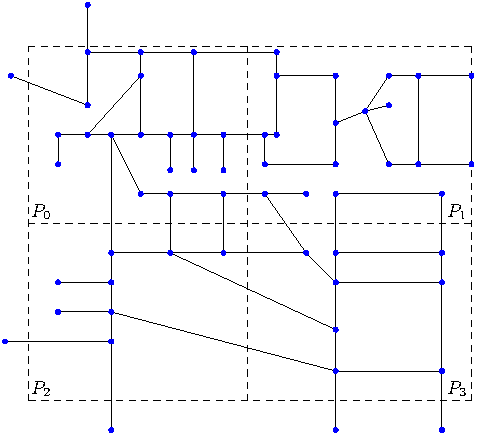
\includegraphics[width=0.49\textwidth]{chapterExtension/model/input/input} &
         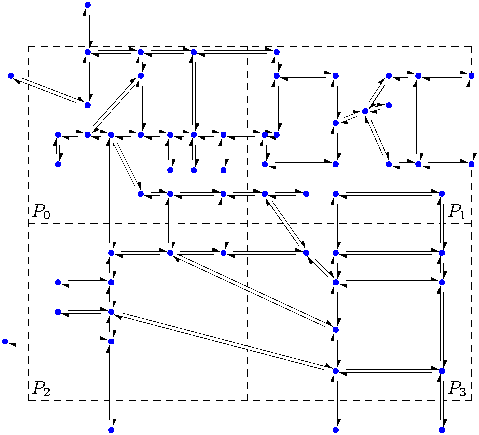
\includegraphics[width=0.49\textwidth]{chapterExtension/model/a/a} \\
         (a) & (b) \\
         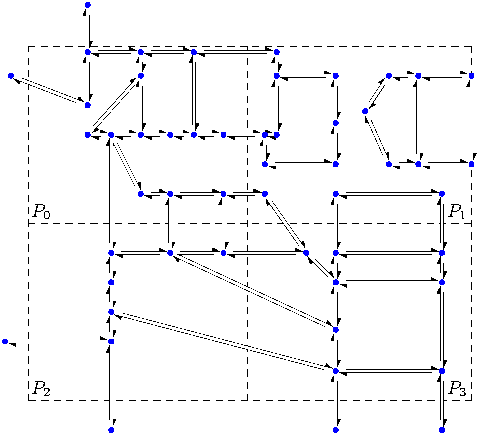
\includegraphics[width=0.49\textwidth]{chapterExtension/model/b/b} &
         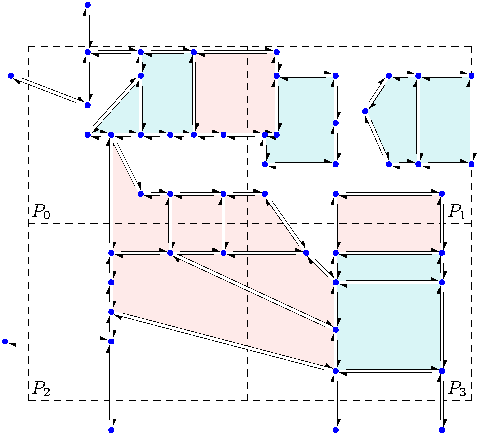
\includegraphics[width=0.49\textwidth]{chapterExtension/model/c/c} \\
         (c) & (d) \\
     \end{tabular}
     \caption{An example of four leaf nodes in a quadtree constructed for input spatial line segments. Solid lines represent the line segments, while dashed lines indicate the Minimum Bounding Rectangles (MBRs) of the partitions. (a) shows the partitioned input spatial lines. (b) shows the DCEL vertices and half-edges. (c) the resulting DCEL after  dangle and cut edge removal.  Finally, (d) shows the final DCEL faces. (taken from \cite{abdelhafeez_ddcel_2023}).} \label{fig:polygonization}
 \end{figure}

 \begin{figure}
    \centering
    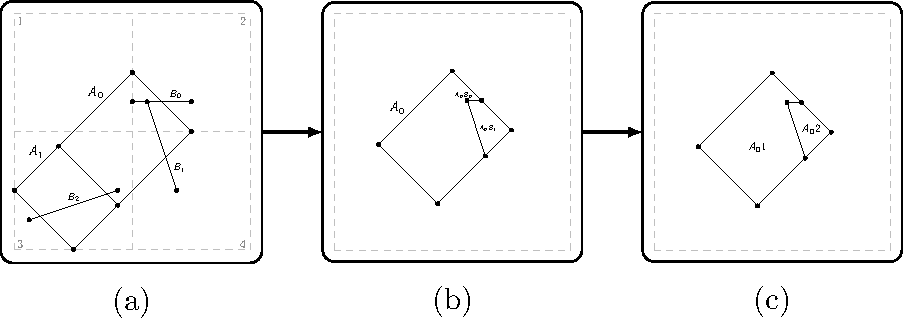
\includegraphics[width=\textwidth]{chapterExtension/dangles_cuts/DAC}
    \caption{(a) Spatial partitioning of input layers A and B, (b) Re-Partitioning of polygon $A_0$ with edges it intersects with, and (c) the result of polygonization of $A_0$ with $B_0, B_1, B_2$.} \label{fig:dangles_cuts}
 \end{figure}

 Figure \ref{fig:dangles_cuts}(a) illustrates the spatial partitioning of two input layers, $A$ and $B$. Layer $A$ contains two input polygons, $A_0$ and $A_1$, while Layer $B$ includes of three dangle edges, $B_0$, $B_1$, and $B_2$.
 
 Each edge in layer $B$ is assigned a unique label and provided as input to the overlay module.  The local overlay processs indentifies intersections between the input polygon layer $A$ and layer $B$ within each data partition.  If a polygon with $id = i$ from layer $A$ intersects with edges labeled $id = a$, $id = b$ and $id = c$ from layer $B$ in a given partition, a composite label $A_{i} B_{a} B_{b} B_{c}$ is generated to represent these intersections.  
 
During the reduce phase, we re-partition the data based on the first label, consolidating all edges that intersect with it. For instance, if two data partitions generate the labels $A_{i} B_{a} B_{b} B_{c}$ and $A_{i} B_{x} B_{y}$, we reassign the data so that $A_{i}$ is grouped within a single partition along with all intersecting edges, specifically $B_{a}, B_{b}, B_{c}, B_{x}, B_{y}$.  In Figure \ref{fig:dangles_cuts}(b), polygon $A_0$ is re-partitioned with the edges it intersects, namely $B_0$, $B_1$, and $B_2$.

After re-partitioning, all intersecting edges from both layers are consolidated within the same partition. The next step is to identify the polygons formed by these intersections. Since there is no guarantee that only one polygon will be generated, we replace the polygon concatenation method proposed in Section \ref{sec:optimizing} with a \textit{polygonization} procedure within each partition. This polygonization process ensures that all possible new polygons are generated.

The polygonization procedure follows the algorithm outlined in \cite{abdelhafeez_ddcel_2023}. It begins by generating new vertices and half-edges, marking the current dangle and cut edges, setting the next pointers, and finally constructing the partition polygons. Figure \ref{fig:dangles_cuts}(c) illustrates the result of polygonizing the edges from polygon$A_0$ and $B_0$, $B_1$, and $B_2$, yielding two polygons,$A_01$ and $A_02$.  The polygons generated from all partitions together form the overlay between polygon layer $A$ and layer $B$.

\section{Experimental Evaluation} \label{sec:experiments}
For our experimental evaluation, we used a 12-node Linux cluster (kernel 3.10) and Apache Spark 2.4. Each node has 9 cores (each core is an Intel Xeon CPU at 1.70GHz) and 2G memory.

The scalable approach was implemented over the Apache Spark framework.  From a Map-Reduce point of view the stages described in Section \ref{sec:methods} were implemented using several transformations and actions supported by Apache Spark.  For example, the partitioning and load balancing described in Section \ref{sec:pstrategies} was implemented using a quadtree, where its leaves were used to map and balance the number of edges that have to be sent to the worker nodes.  Mostly, map operations were used to process and locate the edges in the corresponding leaf to exploit proximity among them while at the same time dividing the amount of work among worker nodes.

Similarly, the edges at each partition were processed using chains of transformations at local level (see Section \ref{sec:methods}) followed by reducer actions to post-process incomplete faces which could span over multiples partitions and have to be combined or re-distributed to obtain the final answer.  In addition, the reduce actions were further optimized as described in Section \ref{sec:alternative_methods}.

\subsection{Evaluation datasets}
The details of the real datasets of polygons that we use are summarized in Table \ref{tab:sdcel_datasets}. The first dataset (MainUS) contains the complete Census Tracts for all the states on the US mainland for the years 2000 (layer A) and 2010 (layer B). It was collected from the official website of the United States Census Bureau \cite{census_tract}. The data was clipped to select just the states inside the continent. Something to note with this dataset is that the two layers present a spatial gap (which was due to improvements in the precision introduced for 2010). As a result, there are considerably more intersections between the two layers, thus creating many new faces for the DCEL.

\begin{table}
    \centering
    \caption{Evaluation Datasets}
    \label{tab:sdcel_datasets}
    \begin{tabular}{c c c c}
        \toprule
        Dataset & Layer & Number        & Number    \\
                &       & of polygons   & of edges  \\
        \midrule
        MainUS& Polygons for 2000 & 64983 & 35417146        \\
              & Polygons for 2010 & 72521 & 36764043        \\
        GADM  & Polygons for Level 2 & 160241 & 64598411    \\
              & Polygons for Level 3 & 223490 & 68779746    \\
        CCT   & Polygons for 2000 & 7028 & 2711639          \\
              & Polygons for 2010 & 8047 & 2917450          \\
        \bottomrule
    \end{tabular}
\end{table}

The second dataset, GADM - taken from Global Administration Areas \cite{gadm_data}, collects the geographical boundaries of the countries and their administrative divisions around the globe. For our experiments, one layer selects the States (administrative level 2), and the other has Counties (administrative level 3). Since GADM may contain multi-polygons, we split them into their individual polygons.

Since these two datasets are too large, a third, smaller dataset was created for comparisons with the sequential algorithm. This dataset is the California Census Tracts (CCT), a subset from MainUS for the state of California; layer A corresponds to the CA census tracts from the year 2000, while layer B corresponds to 2010. Below, we also use other states to create datasets with different numbers of faces.  To test the scalable approach, a sequential algorithm for DCEL creation was implemented based on the pseudo-code outlined in \cite{berg_computational_2008}.

\subsection{Overlay face optimizations}\label{sec:overlay_optimization}
We first examine the optimizations in Section \ref{sec:optimizing}. To consider different distributions of faces, for these experiments, we used 8 states from the MainUS dataset with different numbers of tracts (faces). In particular, we used, in decreasing order of number of tracts, CA, TX, NC, TN, GA, VA, PA, and FL. For each state, we computed the distributed overlay between two layers (2000 and 2010). For each computation, we compared the baseline; master at the root node, with intermediate reducers at different levels: $i$ varied from 4 to 10. 

Figure \ref{fig:overlay_tester} shows the results for the distributed overlay computation stage; after the local DCELs were computed at each cell. 
Note that for each state experiment, we tested different numbers of cells for the quadtree and reported the configuration with the best performance. To determine this, we sampled 1\% of the edges for each state and evaluated the best number of cells ranging from 200 to 2000. In most cases, the best number of cells was around 3000.
As expected, there is a trade-off between parallelism and how much work is left to the final reduce job. For different states, the optimal $i$ varied between levels 4 and 6. The figure also shows the optimization that re-partitions the faces by label id. This approach has actually the best performance. This is because few faces with the same label can be combined independently. This results in smaller jobs better distributed among the cluster nodes, and no reduce phase is needed. As a result, we use the label re-partition approach for the rest of the experiments to implement the overlay computation stage.

\begin{figure}
    \centering
    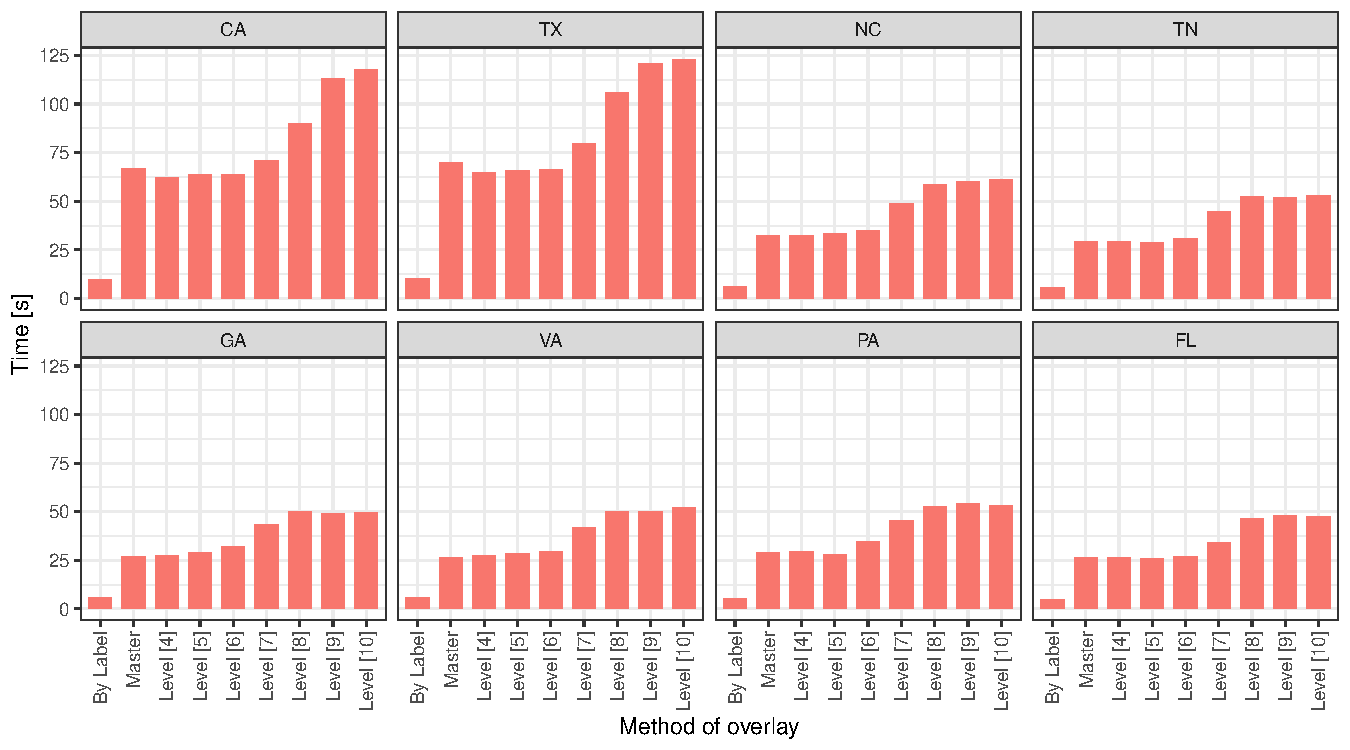
\includegraphics[width=\linewidth]{chapterSDCEL/OverlayTester/Overlay_Tester}
    \caption{Overlay methods evaluation.}\label{fig:overlay_tester}
\end{figure}

Finally we note that the overlay face optimizations involve shuffling of the incomplete faces. Table \ref{tab:percentages} shows the percentage of incomplete faces for three states, assuming 3000 cells. As it can be seen, the incomplete faces is small (in average 12.89\%) and moreover, for the \textit{By-Label} approach, this shuffling is parallelized.

\begin{table}
    \centering
    \caption{Percentages of edges in incomplete faces for three states} \label{tab:percentages}
    \begin{tabular}{cccc}
        \toprule
                & Number of & Edges in         &            \\
        Dataset & edges     & incomplete faces & Percentage \\
        \midrule
        CA &  47834 &  6339 & 13.25\% \\
        TX &  41227 &  4436 & 10.75\%\\
        FL &  24152 &  3547 & 14.68\%\\
        \bottomrule
    \end{tabular}
\end{table}

\subsection{Unbalanced layers optimization}
For these experiments, we compared the traditional sweep approach with the `filtered-sweep' approach that considers only the areas where the smaller layer has edges (Section \ref{sec:unbalance}).  To create the smaller cell layer, we picked a reference point in the state of Pennsylvania, from the MainUS dataset, and added 2000 census tracts until the number of edges reached 3K. We then varied the size of the larger cell layer in a controlled way: using the same reference point but using data from the 2010 census, and we started adding tracts to create a layer that had around 2x, 3x, ..., 7x the number of edges of the smaller dataset.

Since this optimization occurs per cell, we used a single node to perform the overlay computation within that cell. Figure \ref{fig:unbalance_tests}(a) shows the behavior of the two methods (filtered-sweep vs. traditional sweep) under the above-described data for the overlay computation stage.  Clearly, as the data from one layer grows much larger than the other layer, the filtered-sweep approach overcomes the traditional one.

\begin{figure}
    \centering
    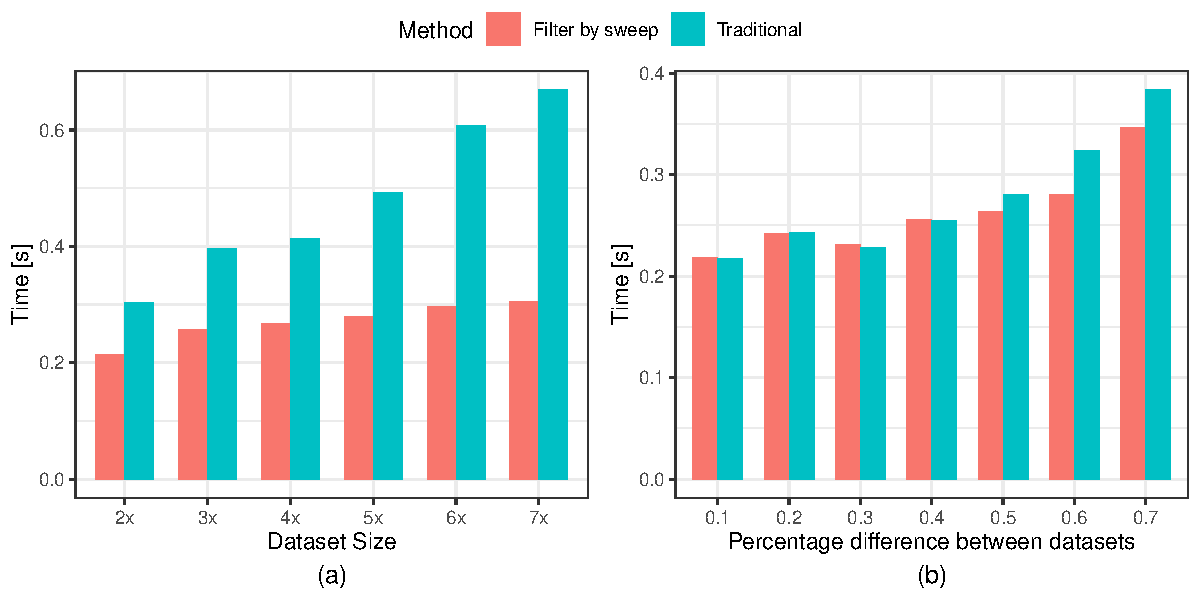
\includegraphics[width=\linewidth]{chapterSDCEL/UnbalanceTester/Unbalance_Tester}
    \caption{Evaluation of the unbalanced layers optimization.}\label{fig:unbalance_tests}
\end{figure}

We also performed an experiment where the difference in size between the two layers varies between 10\% and 70\%. For this experiment, we first identified cells from the GADM dataset where the smaller layer had around 3K edges. Among these cells, we then identified those where the larger layer had 10\%, 20\%, ... up to 70\% more edges. In each category, we picked 10 representative cells and computed the overlay for the cells in that category.

Figure \ref{fig:unbalance_tests}(b) shows the results; in each category, we show the average time to compute the overlay among the 10 cells in that category.  The filtered-sweep approach shows better performance as the percentage difference between layers increases. Based on these results, one could apply the optimization on those cells where the layer difference is significant (more than 50\%).  We anticipate that this optimization will be particularly beneficial for datasets where the two input layers contain many cells with significantly different edge counts.

\subsection{Varying the number of cells}
The quadtree configuration allows for performance tuning by setting the \textit{maximum capacity} of a cell. The quadtree continues splitting until this capacity is reached. There is an inverse relationship between the capacity and the number of leaf cells: a lower capacity results in more cells, while a higher capacity leads to fewer leaf cells. In skewed datasets, the quadtree may become unbalanced, with some branches splitting more frequently. As a result, the final number of partitions is not necessarily a multiple of four. In the figures, we round the number of leaf cells to the nearest thousand.

The number of cells affects the performance of our scalable overlay implementation, termed as SDCEL, since it relates to the average cell capacity given by the number of edges it could contain. As it was said before, a fewer number of cells implies larger cell capacity and thus more edges to process within each cell.  Complementary, creating more cells increases the number of jobs to be executed.

Figure \ref{fig:ca}(a) shows the SDCEL performance using the two layers of the CCT dataset while varying the number of cells from 100 to 15K (by multiple of 1000). Each bar corresponds to the time taken to create the DCEL for each layer and then combine them to create the distributed overlay. Clearly, there is a trade-off: as the number of cells increases, the SDCEL performance improves until a point where the larger number of cells adds an overhead. Figure \ref{fig:ca}(b) focuses on that area; the best SDCEL performance was around 7K cells.

In addition, Figure \ref{fig:ca}(a) shows the performance of the sequential solution (CGAL library) for computing the overlay of the two layers in the CCT dataset using one of the cluster nodes. Clearly, the scalable approach is much more efficient as it takes advantage of parallelism. Note that the CGAL library would crash when processing the larger datasets (MainUS and GADM).

\begin{figure}
    \centering
    \begin{tabular}{cc}
        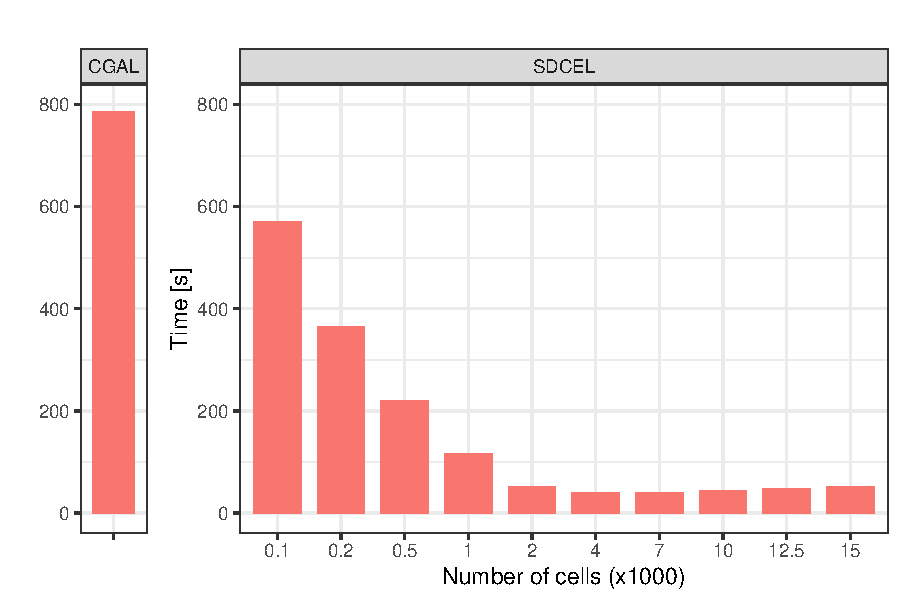
\includegraphics[width=0.50\linewidth]{chapterSDCEL/CA/CA} & 
        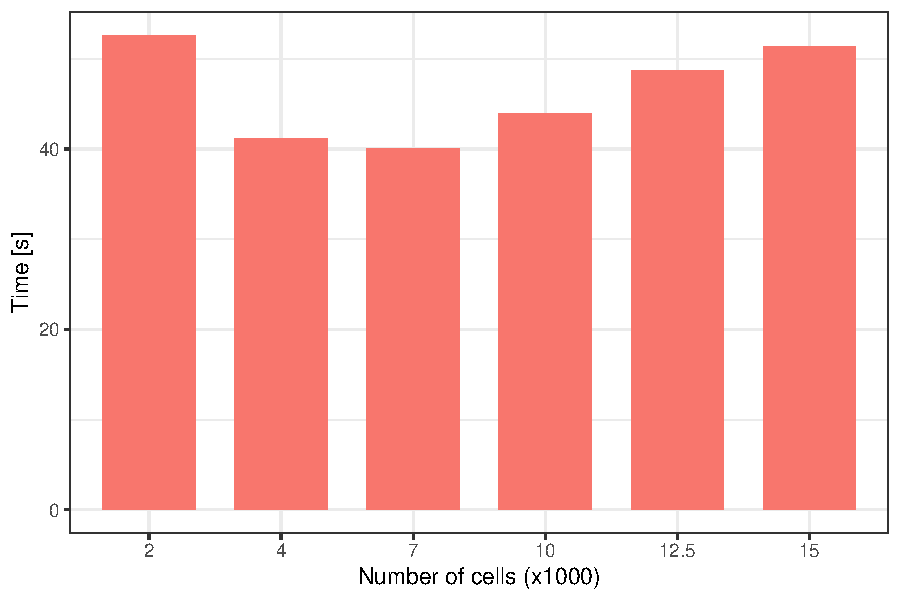
\includegraphics[width=0.45\linewidth]{chapterSDCEL/CA/CA_sample} \\
        (a) & (b)
    \end{tabular}
    \caption{SDCEL performance while varying the number of cells in the CCT dataset.} \label{fig:ca}
\end{figure}

\begin{figure}
    \centering
    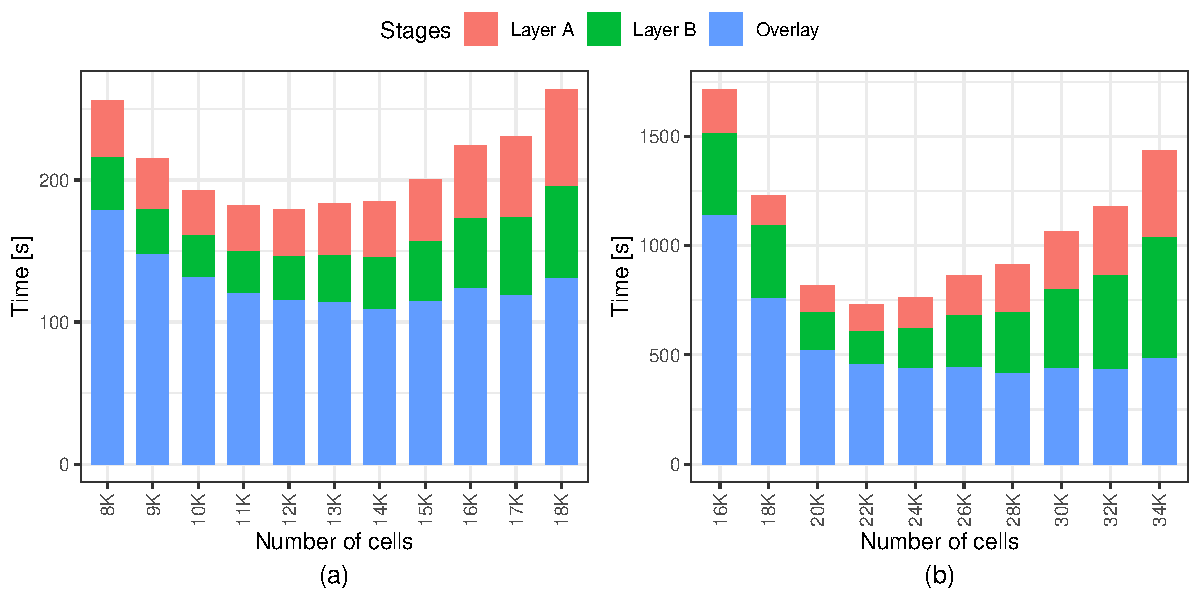
\includegraphics[width=\textwidth]{chapterSDCEL/Performance/Performance} 
    \caption{Performance with (a) MainUS and (b) GADM datasets.} \label{fig:mainus}
\end{figure}

Figure \ref{fig:mainus} shows the results when using the larger MainUS and GADM datasets, while again varying the number of cells parameter from 8K to 18K and from 16K to 34K, respectively. In this figure, we also show the time taken by each stage of the overlay computation.  This is, the time to create the DCEL for layer A, for layer B, and for their combination to create their distributed overlay. We can see a similar trade-off in each of the stages. The best performance is given when setting the number of cells parameter to 12K for the MainUS and 22K for the GADM dataset. Note that in the MainUS dataset, the two layers have a similar number of edges; as can be seen, their DCEL computations are similar.

Interestingly, the overlay computation is expensive since as mentioned earlier there are many intersections between the two layers. An interesting observation from the GADM plots is that layer B takes more time than layer A; this is because there are more edges in the counties than in the states. Moreover, county polygons are included in the (larger) state polygons. When the size of cells is small (i.e., a larger number of cells like in the case of 34K cells), these cells mainly contain counties from layer B. As a result, there are not many intersections between the layers in each cell, and the overlay computation is thus faster. On the other hand, with large cell sizes (smaller number of cells), the area covered by the cell is larger, containing more edges from states and thus increasing the number of intersections, resulting in higher overlay computation.

Additionally, Table \ref{tab:cell_stats} provides statistics on the cells. It shows that in larger datasets, an average cell size of approximately 3000 edges produces the best results. This cell size ensures a relatively small amount of data to transmit, which minimizes the impact on data shuffling and processing.  Table \ref{tab:orphans} presents the number of cells, original holes, and the orphan cells and holes generated after partitioning.

\begin{table}
    \centering
    \caption{Cell size statistics.}
    \label{tab:cell_stats}
    \begin{tabular}{ccccccc}
        \toprule
        Dataset & Min & 1st Qu. & Median & Mean & 3rd Qu. & Max   \\
        \midrule
        GADM    & 0   & 0       & 2768   & 3141 & 5052    & 16978 \\
        MainUS  & 0   & 1538    & 2582   & 2853 & 3970    & 10944 \\
        CCT     & 0   & 122     & 324    & 390  & 546     & 1230  \\
        \bottomrule
    \end{tabular}
\end{table}

\begin{table}
    \centering
    \caption{Orphan cells and orphan holes description}
    \label{tab:orphans}
    \begin{tabular}{c c c c}
        \toprule
                & Number   & Number   & Number of orphans   \\
        Dataset & of cells & of holes & (cell/holes) \\
        \midrule
        GADM  & 21970      & 1999     & 4310 \\
        MainUS& 12343      & 850      & 1069 \\
        CCT   & 7124       & 40       & 215  \\
        \bottomrule
    \end{tabular}
\end{table}

\subsection{Speed-up and Scale-up experiments} \label{sec:speed_scale}
The speed-up behavior of SDCEL appears in Figure \ref{fig:mainus_speed_scale}(a) (for the MainUS dataset) and in Figure \ref{fig:gadm_speed_scale}(a) (for the GADM dataset); in both cases, we show the performance for each stage. For these experiments, we varied the number of nodes to 3, 6, and 12 while keeping the input layers the same. Clearly, as the number of nodes increases, the performance improves. SDCEL shows good speed-up characteristics: as the number of nodes doubles from 3 to 6 and then from 6 to 12, the performance improves by almost half.

\begin{figure}
    \centering
    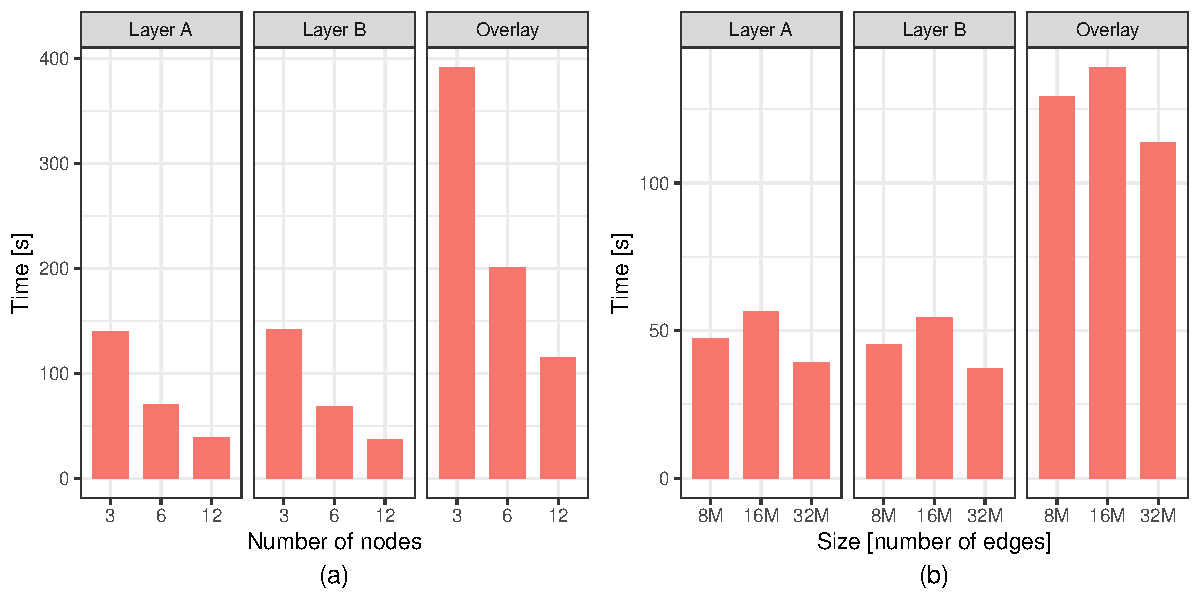
\includegraphics[width=\textwidth]{chapterSDCEL/MainUS_SS/MainUS_SS} 
    \caption{Speed-up and Scale-up experiments for the MainUS dataset.} 
\label{fig:mainus_speed_scale}
\end{figure}

\begin{figure}
    \centering
    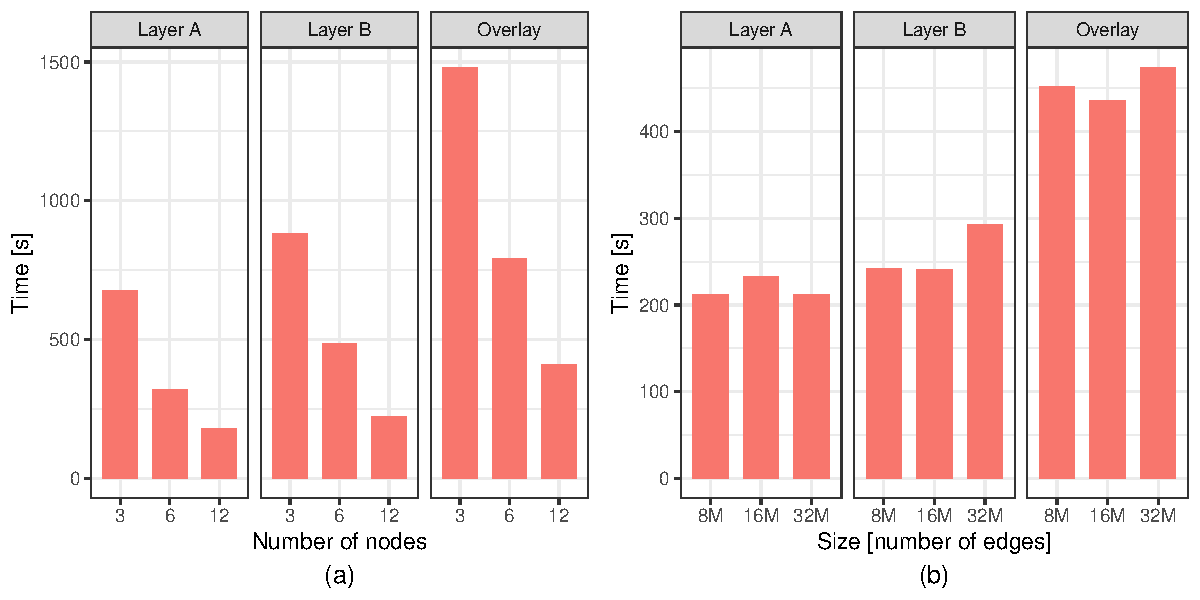
\includegraphics[width=\textwidth]{chapterSDCEL/GADM_SS/GADM_SS}
    \caption{Speed-up and Scale-up experiments for the GADM dataset.} \label{fig:gadm_speed_scale}
\end{figure}

To examine the scale-up behavior, we created smaller datasets out of the MainUS and similarly out of the GADM so that we could control the number of edges. To create such a dataset, we picked a centroid and started increasing the area covered by this dataset until the number of edges was closed to a specific number. For example, from the MainUS, we created datasets of sizes 8M, 16M, and 32M edges for each layer. We then used two layers of the same size as input to a different number of nodes while keeping the input-to-node ratio fixed. That is, the layers of size 8M were processed using 3 nodes, the layers of size 16M using 6 nodes, and the 32M using 12 nodes. We used the same process for the scale-up experiments with the GADM dataset. The results appear in Figure \ref{fig:mainus_speed_scale}(b) and Figure \ref{fig:gadm_speed_scale}(b).  Overall, SDCEL shows good scale-up performance; it remains almost constant as the work per node is similar (there are slight variations because we could not control perfectly the number of edges and their intersection).

%% Extension
%\subsection{Kd-tree versus quadtree performance} \label{sec:comparison}
%In order to compare the quadtree and the kd-tree partition strategies we analyze their performance during the construction of the spatial data structure which defines the cells that the partition will use based on the sample, the cost of partitioning; populating the cells with the full datasets, and the overall time to complete the phases of the overlay operation using each partitioning approach.  We use the datasets of MainUS and GADM described in Table \ref{tab:datasets}.

% \begin{figure}
%     \centering
%     \begin{tabular}{cc}
%         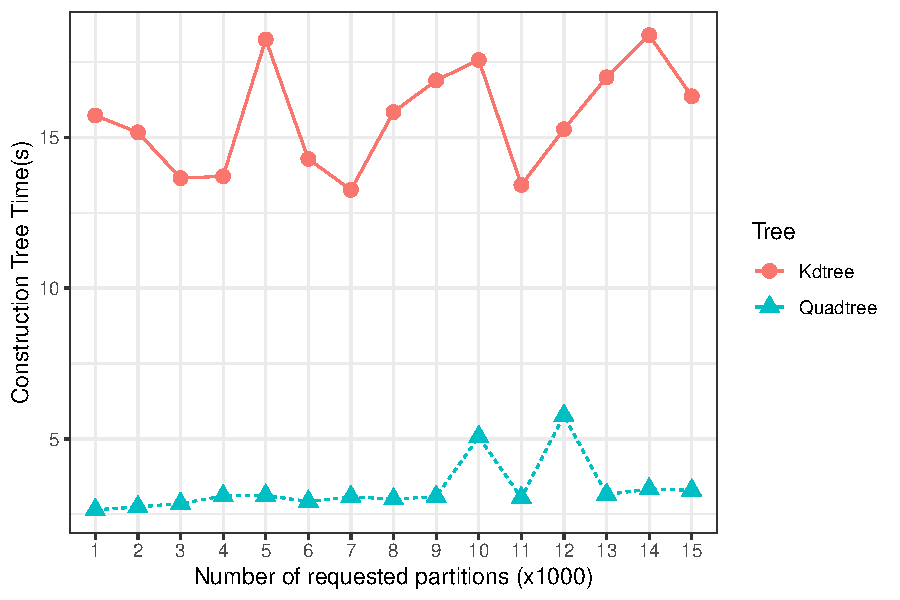
\includegraphics[width=0.49\linewidth]{chapterSDCEL/K_Creation_US.pdf} & 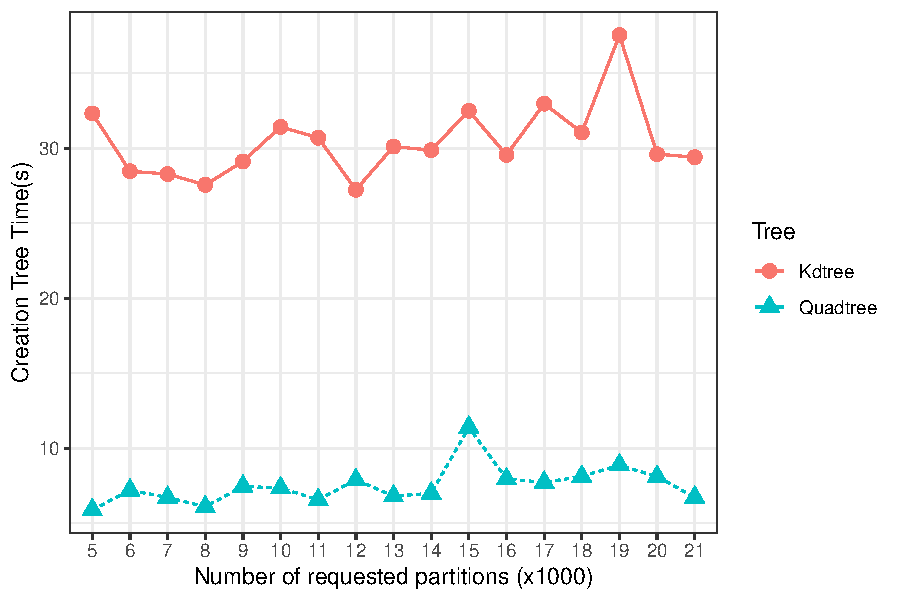
\includegraphics[width=0.49\linewidth]{chapterSDCEL/K_Creation_GADM.pdf} \\
%         (a) & (b)
%     \end{tabular}
%     \caption{Construction time for the spatial data structure in the (a) MainUS and (b) GADM datasets.} \label{fig:k_creation_us}
% \end{figure}

% \begin{figure}
%     \centering
%     \begin{tabular}{cc}
%         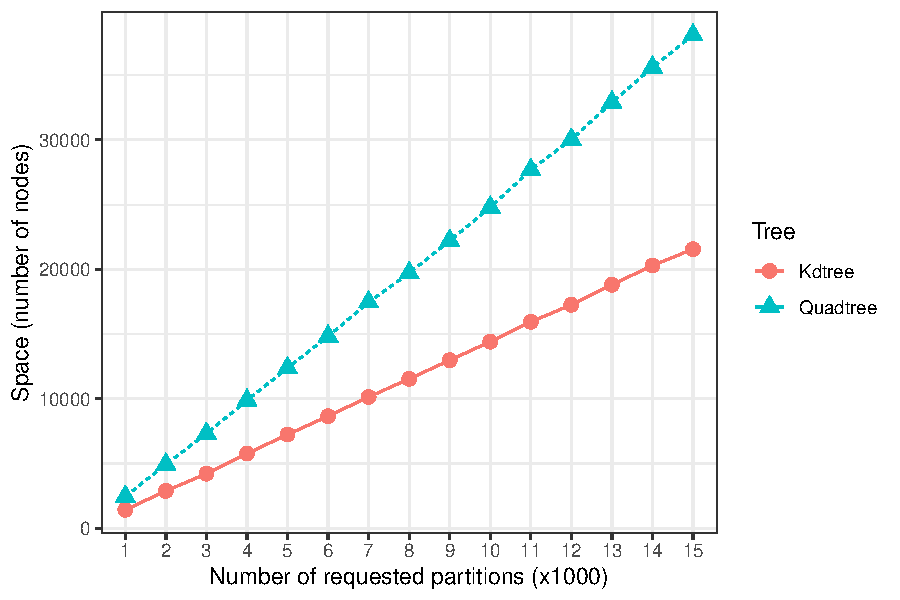
\includegraphics[width=0.49\linewidth]{chapterSDCEL/K_Space_US.pdf} & 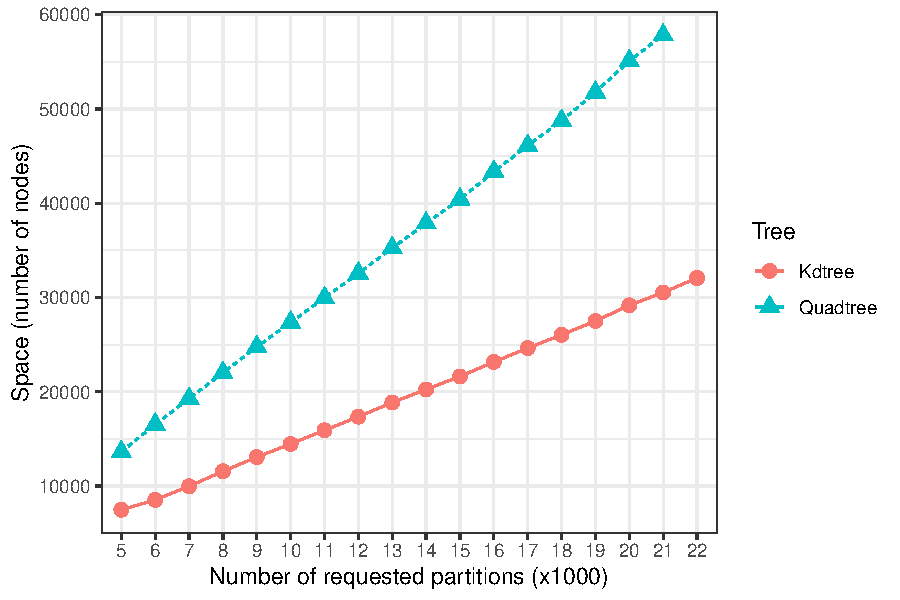
\includegraphics[width=0.49\linewidth]{chapterSDCEL/K_Space_GADM.pdf} \\
%         (a) & (b)
%     \end{tabular}
%     \caption{Number of cells created by each spatial data structure in the (a) MainUS and (b) GADM datasets.} \label{fig:k_space_us}
% \end{figure}

% Figure \ref{fig:k_creation_us} depicts the construction time during the sampling of the input layers and the generation of the partitioning cells after requesting a different number of divisions. We can see that the kd-tree takes more time, particularly because of the sorting done at each split, so as to organize the data and localize the middle point. In average, Quadtree takes 23.13\% the time it takes for Kdtree to be created (21.55\% in MainUS and 24.72\% in GADM). However, the Kdtree creation is just 5.86\% of the overall time during the total DCEL construction (6.88\% in MainUS and 4.87\% in GADM).

% \begin{figure}
%     \centering
%     \begin{tabular}{cc}
%         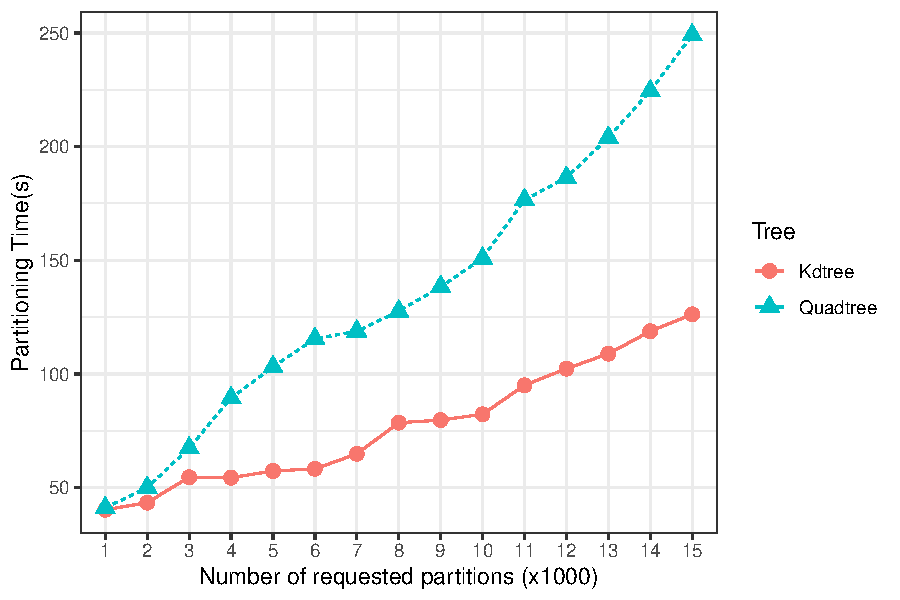
\includegraphics[width=0.49\linewidth]{chapterSDCEL/K_Partitioning_US.pdf} &
%         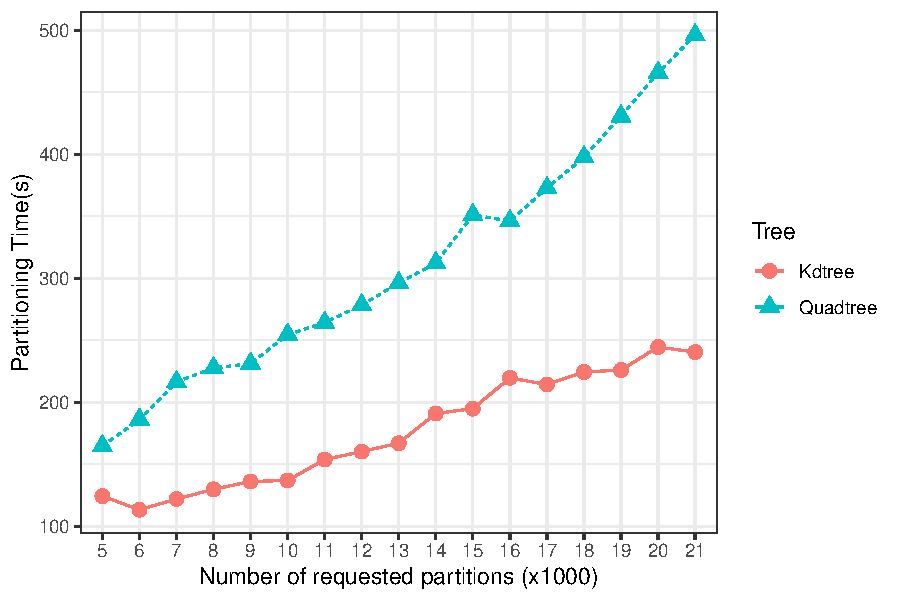
\includegraphics[width=0.49\linewidth]{chapterSDCEL/K_Partitioning_GADM.pdf} \\
%         (a) & (b)
%     \end{tabular}
%     \caption{Data partitioning time using a spatial data structure (a) in the MainUS dataset and (b) in the GADM dataset.} \label{fig:k_partitioning_us}
% \end{figure}

%An important characteristic of the behavior of each partitioning scheme is the number of cells (partitions) each sample data structure creates. Figure \ref{fig:k_space_us} depicts the number of cells created by each spatial data structure. As the quadtree follows a space-oriented technique, it creates more nodes (4 at each split) and thus generates more leaves (cells); more of them are prone to be empty compared to the kd-tree.

%Figure \ref{fig:k_partitioning_us} shows the cost to partition the full content of both layers. Given a sample tree data structure, each edge is assigned to a cell (partition) depending on which leaf the edge is located; edges are assigned (copied) to all leaves they intersect. Then, a shuffle operation is performed to move the data to the corresponding node that will handle this cell (partition). This figure shows that the quadtree partitioning takes more time. This depends largely on the number of leaves created by the sample tree and the number of edges that overlap partitions (which is expected to be larger for the quadtree since it uses more and thus smaller cells).

% \begin{figure}
%     \centering
%     \begin{tabular}{cc}
%         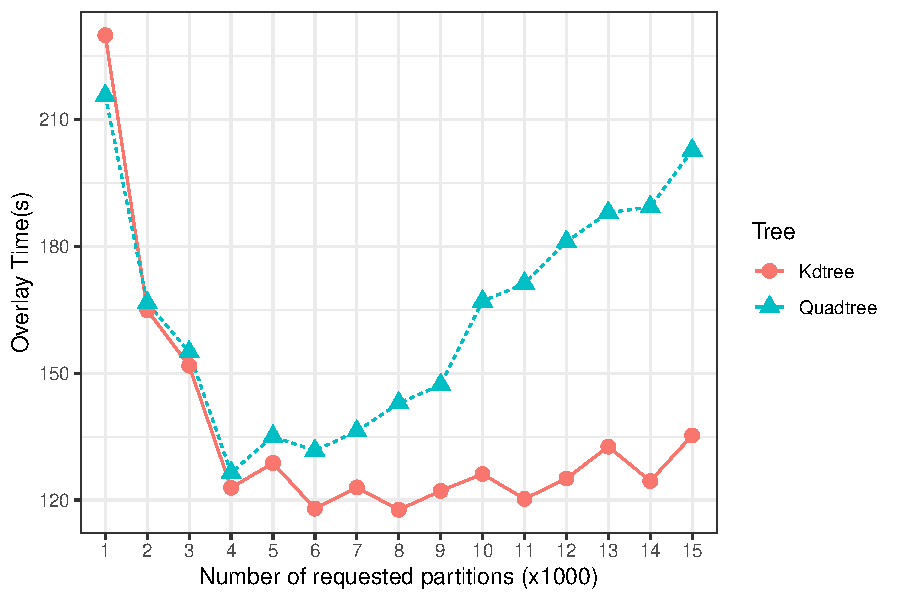
\includegraphics[width=0.49\linewidth]{chapterSDCEL/K_Overlay_US.pdf} &
%         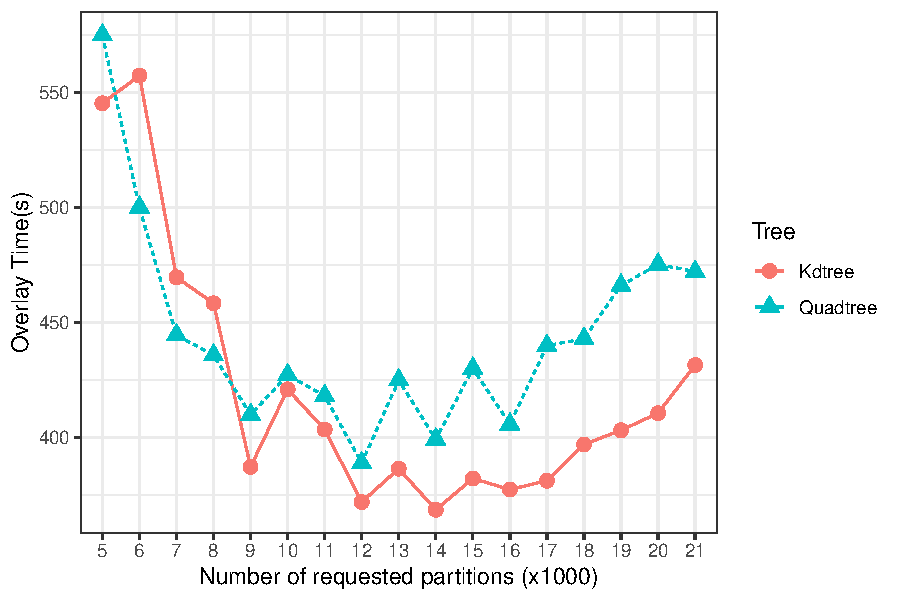
\includegraphics[width=0.49\linewidth]{chapterSDCEL/K_Overlay_GADM.pdf} \\
%         (a) & (b)
%     \end{tabular}
%     \caption{Execution time for the overlay operation using a spatial data structure in the MainUS (a)and GADM (b) dataset.} \label{fig:k_overlay_us}
% \end{figure}

%Once the data is assigned to their partitions, the overlay operation can be executed.  Figure \ref{fig:k_overlay_us} shows the overlay performance under each partition strategy, for different number of cells. The Kd-tree approach performs better; as the quadtree tends to generate more and emptier cells, its performance is directly affected.

%As it was said before, in particular on partitioning based on Kdtree, the smaller number of cells/partitions used in this approach give also an improvement on the impact of shuffling during the partition strategy because the number and size of the resulting partitions have a lower impact into the communication cost.

%Finally, we consider the speed-up and scale-up performance using the kd-tree partitioning. Figure \ref{fig:k_scale_speed_us}(a) shows the speed-up performance using the MainUS dataset (36M edges) while varying the number of nodes (for 3, 6, and 12 nodes). Similar to the quadtree partitioning strategy, the kd-tree partitioning shows good speed-up performance. As resources duplicate the execution time improves almost by a half.

%Figure \ref{fig:k_scale_speed_us}(b) shows the scale-up performance of the kd-tree partitioning approach. We followed the same procedure described in Section \ref{sec:speed_scale} to generate datasets for 8M, 16M, and 32M edges from the MainUS dataset and ran the kd-tree partitioning strategy with 3, 6, and 12 nodes, respectively. Again the kd-tree partitioning shows good speed-up performance, which remains flat as the load per node is almost equal.

% \begin{figure}
%     \centering
%     \begin{tabular}{cc}
%         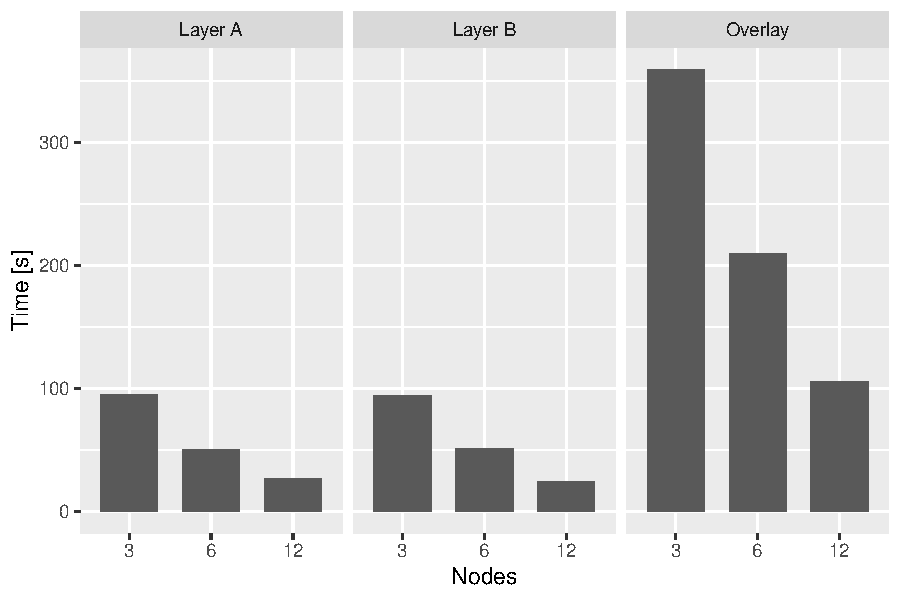
\includegraphics[width=0.49\linewidth]{chapterSDCEL/US_speedup.pdf} & 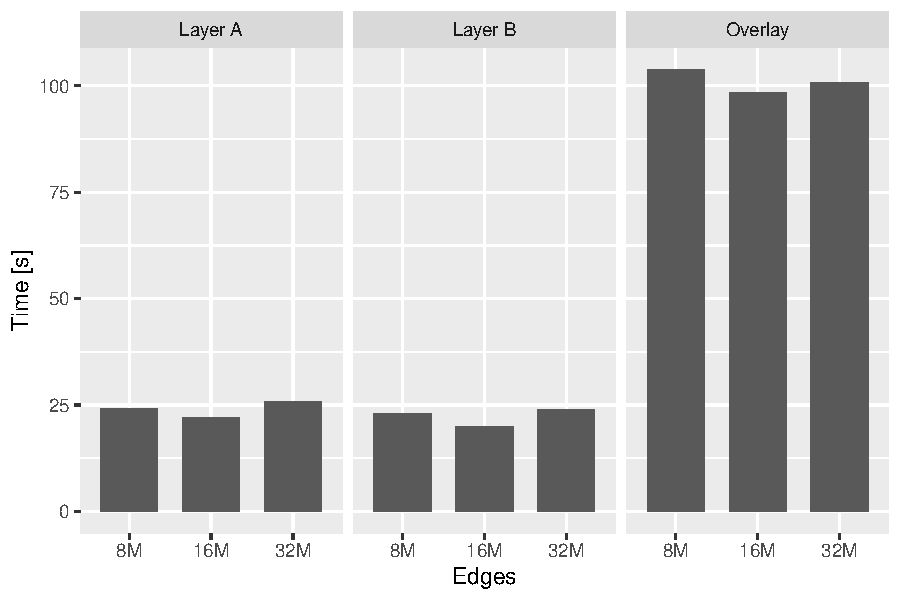
\includegraphics[width=0.49\linewidth]{chapterSDCEL/US_scaleup.pdf} \\
%         (a) & (b)
%     \end{tabular}
%     \caption{(a)Speed Up and (b) Scale Up performance of the Kdtree partitioning using the MainUS dataset.} \label{fig:k_scale_speed_us}
% \end{figure}


%% Extension
%\subsection{Polygonization Scalability}\label{sec:expr:query}
% \begin{table}
%     \centering
%     \caption{Polygonization Evaluation Dataset}
%     \label{table:polygonization:datasets}
%     \begin{tabular}{c c c c c}
%         \toprule
%         Dataset  & Area & Number of Line Segments & Faces \\
%         \midrule
%         USA & 9.83 $Mkm^2$ & 152$M$ & 5$M$ \\
%         South America & 17.8 $Mkm^2$ & 155$M$ & 7$M$\\
%         North America & 24.7 $Mkm^2$ & 240$M$ & 10$M$ \\
%         Africa & 30.4 $Mkm^2$ & 288$M$ & 10$M$  \\
%         Europe & 10.2 $Mkm^2$ & 563$M$ & 25$M$ \\
%         Asia & 44.6 $Mkm^2$ & 557$M$ & 23$M$ \\
%         \bottomrule
%     \end{tabular}
% \end{table}

% \begin{figure}
% \centering
% 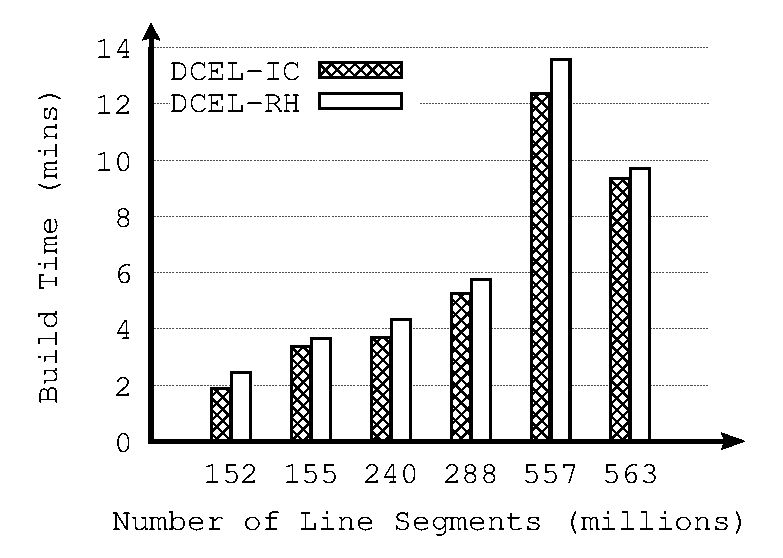
\includegraphics[width=0.48\linewidth]{chapterSDCEL/Experiments/n_records.eps}
% 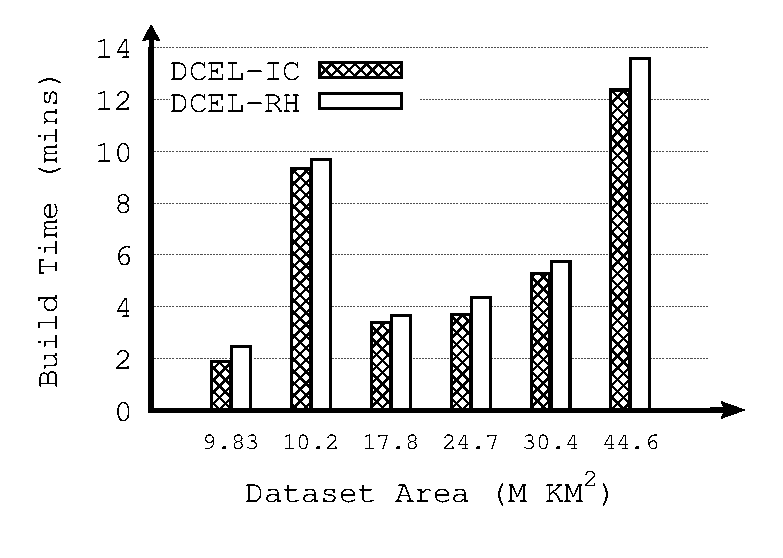
\includegraphics[width=0.48\linewidth]{chapterSDCEL/Experiments/area.eps}
% \caption{Polygonization Performance on Real Road Networks.}
% \label{fig:exp:query}
% \end{figure}

%Figure \ref{fig:exp:query} evaluates the scalability of the polygonization approach using the different evaluation datasets summarized in Table \ref{table:polygonization:datasets}.  We implemented our polygonization framework on Apache Sedona \cite{yu_spatial_2018}. The experiment is based on a Java 8  implementation and utilizes a Spark 2.3 cluster with two driver nodes and 12 worker nodes. All nodes run Linux CentOS 8.2 (64-bit). Each driver node is equipped with 128GB of RAM, while each worker node has 64GB of RAM. To increase parallelism, we divided the 12 worker nodes into 84 worker executors. Each executor is a separate JVM process with dedicated resources, such as memory and CPU cores. The distribution of these executors across the nodes is managed by the resource negotiator (YARN), which allocates resources for Spark jobs based on the availability of cores and memory. YARN typically balances resources across the cluster, so executors are likely to be evenly distributed, though some variation may occur due to resource availability at runtime. Assuming an even distribution, each worker node would run approximately 7 executors, as calculated by $\frac{84}{12} = 7$.

%As discussed in Section \ref{sec:rem}, the Rem Phase has two different approaches depending on the input data received from the Gen Phase. The first approach is to process the remaining half-edges iteratively, denoted as \textit{DCEL-RH}. In comparison, the second approach processes the incomplete cycles generated from the first phase iteratively denoted as \textit{DCEL-IC}.

%From Figure \ref{fig:exp:query}, we draw three conclusions; (1) first, the cardinality of the input dataset has a positive correlation with the build time; as the number of line segments increases, the build time also increases, as shown in Figure \ref{fig:exp:query}(a). However, we see that we have close cardinality for Asia (557M) and Europe (563M) datasets, but there is a noticeable difference in the build time; moreover, the build time for the Europe dataset is less than that of the Asia dataset. This drives us to the second conclusion; (2) for datasets with close or similar cardinalities, the area of the dataset has a positive correlation with the build time shown in Figure \ref{fig:exp:query}(b). Hence the build time of the Europe dataset (10.2 $Mkm^2$) is less than that of the Asia dataset (44.6 $Mkm^2$), even though Europe has a slightly larger dataset.  (3) The third conclusion is that for all evaluated datasets, the \textit{DCEL-IC} beats \textit{DCEL-RH}.


%% Extension
%\subsection{Polygonization Speed Up Evaluation} \label{sec:expr:speedup}
% \begin{figure}[tb]
% 	\centering
% 	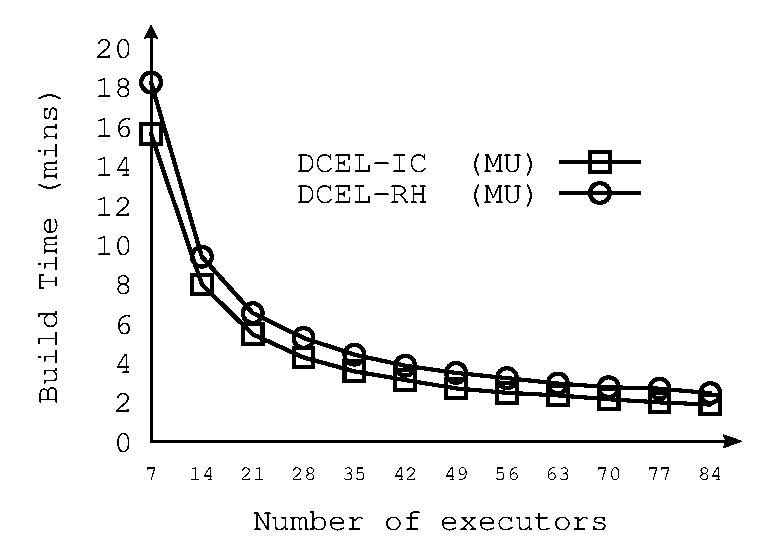
\includegraphics[width=8.8cm]{chapterSDCEL/Experiments/speedup.eps}
% 	\caption{Polygonization speed up evaluation using the USA dataset}
% 	\label{fig:exp:speedup}
% \end{figure}

%Figure \ref{fig:exp:speedup} shows the effect of increasing the number of executors on the build time for the USA dataset.  At each step in the figure, we add 7 more executors, which is approximately equivalent to adding one additional node.  Overall, our approach has good speedup performance. As the number of executors is doubled from 7 executors to 14 executors, the build time is almost halved.  This trend goes on as we double the number of executors. As we increase the number of executors from 7 to 84, the build time is decreased by a factor of 8.


%% Extension
%\subsection{Overlaying Polygons with Dangle and Cut Edges}
% \begin{table}
%     \caption{Overlaying Polygons with Dangle and Cut Edges Dataset}
%     \label{tab:dangles}
%     \begin{tabular}{c c c c}
%         \toprule
%         Dataset & Number Layer $A$ of Polygons & Number of Layer $B$ Edges & Result Polygons \\
%         \midrule
%         TN & 1,272 & 3,380,780 & 41,761 \\
%         GA & 1,633 & 4,647,171 & 49,125 \\
%         NC & 1,272 & 7,212,604 & 22,413 \\
%         TX & 4,399  & 8,682,950 & 98,635 \\
%         VA & 1,554 & 8,977,361 & 38,941 \\
%         CA & 7,038 & 9,103,610 & 96,916\\
%         \bottomrule
%     \end{tabular}
% \end{table}

% \begin{figure}
%     \centering
%     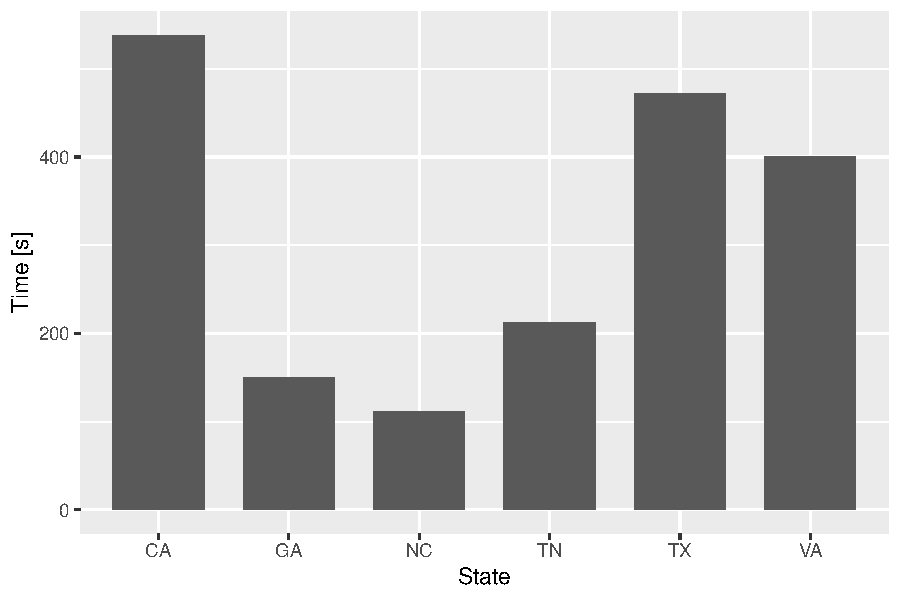
\includegraphics[width=0.7\linewidth]{chapterSDCEL/states.pdf}
%     \caption{Overlaying State polygons with dangle and cut edges.}
%     \label{fig:dangle}
% \end{figure}

%In this section, we examine the performance of overlaying polygons with dangle and cut edges resulting from the polygonization as detailed in Section \ref{sec:over_dang}.  Table \ref{tab:dangles} shows the number of polygons for each state for the first layer of the overlay. It also shows the number of dangle and cut edges per state for the second layer of the overlay. Finally, it shows the number of resultant polygons per state.  From Figure \ref{fig:dangle}, we conclude that the running time is affected by the number of dangle and cut edges and the number of intersections between the two layers (represented by the number of generated polygons).  TN and GA have a relatively smaller number of dangle and cut edges, so they have lower execution times compared to VA, TX, and CA. However, since the intersections in NC are significantly less than those of TN and GA, NC has the lowest execution time. TX, VA, and CA have a comparable number of edges; however, VA has the least number of intersections, resulting in lower execution time compared to TX and CA.

\section{Conclusions} \label{sec:conclusions}
We present a novel, scalable approach to discovering moving flock patterns in large trajectory databases. By leveraging distributed frameworks, the proposed method overcomes the limitations of sequential algorithms that struggle with large-scale spatio-temporal datasets. Through partitioning and replication, as well as improvements in pruning and temporal joins, this approach efficiently handles dense data, offering significant performance improvements over traditional methods. The evaluation results demonstrate the scalability and effectiveness of the approach, making it a valuable contribution for analyzing complex movement patterns.

\bibliographystyle{ACM-Reference-Format}
\bibliography{pflocks, pflock}
\newpage 
\appendix

\section{Center computation.}
\begin{algorithm}
    \caption{Find the centers of given radius which circumference laid on the two input points.}
    \begin{algorithmic}[1]
        \Require Radius $\frac{\varepsilon}{2}$ and points $p_1$ and $p_2$.
        \Ensure Centers $c_1$ and $c_2$.
        
        \Function{FindCenters}{$p_1$, $p_2$, $\frac{\varepsilon}{2}$}
        \State $r^2 \gets (\frac{\varepsilon}{2})^2$
        \State $X \gets p_1.x - p_2.x$
        \State $Y \gets p_1.y - p_2.y$
        \State $d^2 \gets X^2 + Y^2$
        \State $R \gets \sqrt{\lvert 4 \times \frac{r^2}{d^2} - 1 \rvert}$
        \State $c_1.x \gets X + \frac{Y \times R}{2} + p_2.x$
        \State $c_1.y \gets Y - \frac{X \times R}{2} + p_2.y$
        \State $c_2.x \gets X - \frac{Y \times R}{2} + p_2.x$
        \State $c_2.y \gets Y + \frac{X \times R}{2} + p_2.y$
        
        \State \Return $c_1$ and $c_2$
        \EndFunction
    \end{algorithmic}
    \label{app:centers}
\end{algorithm}

\section{Disk pruning.}
\begin{algorithm}
    \caption{Prune disks which are duplicate or subset of others.}
    \begin{algorithmic}[1]
        \Require Set of disks $D$.
        \Ensure Set of disks $D^{\prime}$ without duplicate or subsets.
        
        \Function{PruneDisks}{$D$}
        \State $E \gets \varnothing$
        \ForAll{disk $d_i$ in $D$}
            \State $N \gets d_i \cap D$
            \ForAll{disk $n_j$ in $N$}
                \If{$d_i$ contains all the elements of $n_j$}
                        \State $E \gets E \cup {n_j}$
                \EndIf
            \EndFor
        \EndFor        
        \State $D^{\prime} \gets D \setminus E$
        \State \Return $D^{\prime}$
        \EndFunction
    \end{algorithmic}
    \label{app:disks}
\end{algorithm}

\section{Clique and MBC approach.}
\begin{figure}
    \centering
    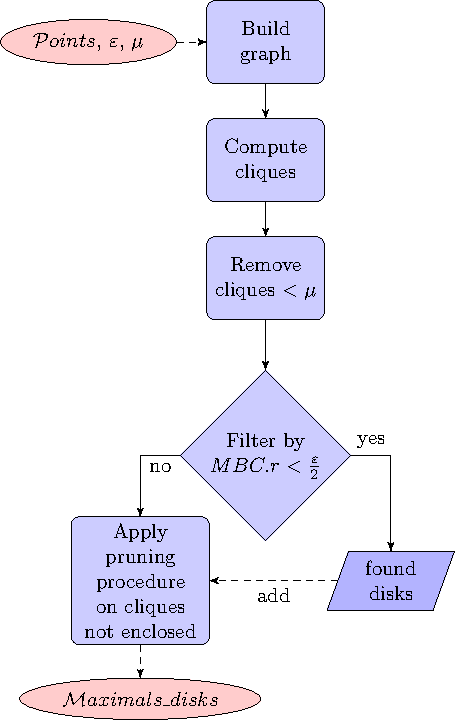
\includegraphics[width=0.7\linewidth]{figures/plots/10_cmbc_variants/CMBC_flowchart2.pdf}
    \caption{Schematic description of the Clique and MBC approach.}
    \label{fig:cmbc_flowchart}
\end{figure}

\end{document}
